\documentclass{beamer}

\usetheme{Darmstadt}
\usecolortheme{crane}

\usepackage[T1]{fontenc}
\usepackage{eurosym}
\usepackage{lmodern}
\usepackage[utf8]{inputenc}
\usepackage[french]{babel}

\title{Frameworks de développement cross-platform}
\subtitle{L'avenir du développement mobile ?}
\author{Thibaud Destouches \& Marceau Lacroix}
\date{}
\institute{ISTIC -- Université de Rennes 1}

\begin{document}

\begin{frame}[fragile]
\titlepage
\end{frame}

\begin{frame}
\setcounter{tocdepth}{2}
\tableofcontents
\end{frame}

\section{Introduction}
\subsection{Problématique}

\begin{frame}
  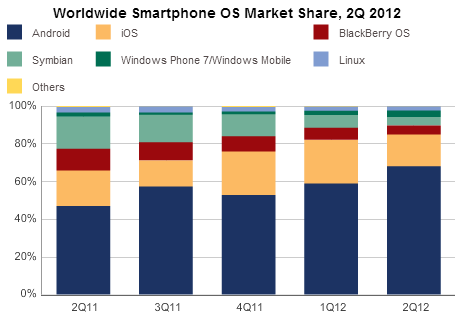
\includegraphics[scale=0.9]{segm}
\end{frame}

\subsection{Enjeux}

\begin{frame}
\textbf{Un secteur en grande progression...}
\\ ~ \\
  \begin{itemize}
    \item Profiter d'un marché de plus en plus importants
    \begin{itemize}
      \item Ventes Smartphones > Ventes PC (2012)
    \end{itemize}
    \item Réduire le Time-to-Market
    \item Limiter la segmentation des OS
    \begin{itemize}
      \item Android (68.1 \%)
      \item iOS (16.9 \%)
      \item BlackBerry OS (4.8 \%)
      \item Windows Phone (4.4 \%)
      \item ...
    \end{itemize}
    \item Faciliter la maintenabilité
  \end{itemize}
\end{frame}


\section{Etat de l'art}

\subsection{Compilation Web}
\begin{frame}
\end{frame}

\subsection{Compilation native}
\begin{frame}
\end{frame}

\section{Conclusion}
\begin{frame}{Conclusion}
\begin{columns}[c]
  \begin{column}{0.5\textwidth}
    \textbf{Avantages}
    \begin{itemize}
      \item Réduction du temps de développement
      \item Maintenabilité facilité
    \end{itemize}
  \end{column}
  \begin{column}{0.5\textwidth}
    \textbf{Inconvénients}
    \begin{itemize}
      \item Limitation des APIs
      \item Compilation Web
      \item Code généré de qualité inférieur à un développement spécifique
      \item Non support de certains matériels
      \item Prix de la licence
    \end{itemize}
  \end{column}
\end{columns}
\end{frame}


\end{document}
